% Options for packages loaded elsewhere
% Options for packages loaded elsewhere
\PassOptionsToPackage{unicode}{hyperref}
\PassOptionsToPackage{hyphens}{url}
\PassOptionsToPackage{dvipsnames,svgnames,x11names}{xcolor}
%
\documentclass[
  11pt,
  letterpaper,
]{article}
\usepackage{xcolor}
\usepackage[margin=1in]{geometry}
\usepackage{amsmath,amssymb}
\setcounter{secnumdepth}{5}
\usepackage{iftex}
\ifPDFTeX
  \usepackage[T1]{fontenc}
  \usepackage[utf8]{inputenc}
  \usepackage{textcomp} % provide euro and other symbols
\else % if luatex or xetex
  \usepackage{unicode-math} % this also loads fontspec
  \defaultfontfeatures{Scale=MatchLowercase}
  \defaultfontfeatures[\rmfamily]{Ligatures=TeX,Scale=1}
\fi
\usepackage{lmodern}
\ifPDFTeX\else
  % xetex/luatex font selection
\fi
% Use upquote if available, for straight quotes in verbatim environments
\IfFileExists{upquote.sty}{\usepackage{upquote}}{}
\IfFileExists{microtype.sty}{% use microtype if available
  \usepackage[]{microtype}
  \UseMicrotypeSet[protrusion]{basicmath} % disable protrusion for tt fonts
}{}
\makeatletter
\@ifundefined{KOMAClassName}{% if non-KOMA class
  \IfFileExists{parskip.sty}{%
    \usepackage{parskip}
  }{% else
    \setlength{\parindent}{0pt}
    \setlength{\parskip}{6pt plus 2pt minus 1pt}}
}{% if KOMA class
  \KOMAoptions{parskip=half}}
\makeatother
% Make \paragraph and \subparagraph free-standing
\makeatletter
\ifx\paragraph\undefined\else
  \let\oldparagraph\paragraph
  \renewcommand{\paragraph}{
    \@ifstar
      \xxxParagraphStar
      \xxxParagraphNoStar
  }
  \newcommand{\xxxParagraphStar}[1]{\oldparagraph*{#1}\mbox{}}
  \newcommand{\xxxParagraphNoStar}[1]{\oldparagraph{#1}\mbox{}}
\fi
\ifx\subparagraph\undefined\else
  \let\oldsubparagraph\subparagraph
  \renewcommand{\subparagraph}{
    \@ifstar
      \xxxSubParagraphStar
      \xxxSubParagraphNoStar
  }
  \newcommand{\xxxSubParagraphStar}[1]{\oldsubparagraph*{#1}\mbox{}}
  \newcommand{\xxxSubParagraphNoStar}[1]{\oldsubparagraph{#1}\mbox{}}
\fi
\makeatother


\usepackage{longtable,booktabs,array}
\newcounter{none} % for unnumbered tables
\usepackage{calc} % for calculating minipage widths
% Correct order of tables after \paragraph or \subparagraph
\usepackage{etoolbox}
\makeatletter
\patchcmd\longtable{\par}{\if@noskipsec\mbox{}\fi\par}{}{}
\makeatother
% Allow footnotes in longtable head/foot
\IfFileExists{footnotehyper.sty}{\usepackage{footnotehyper}}{\usepackage{footnote}}
\makesavenoteenv{longtable}
\usepackage{graphicx}
\makeatletter
\newsavebox\pandoc@box
\newcommand*\pandocbounded[1]{% scales image to fit in text height/width
  \sbox\pandoc@box{#1}%
  \Gscale@div\@tempa{\textheight}{\dimexpr\ht\pandoc@box+\dp\pandoc@box\relax}%
  \Gscale@div\@tempb{\linewidth}{\wd\pandoc@box}%
  \ifdim\@tempb\p@<\@tempa\p@\let\@tempa\@tempb\fi% select the smaller of both
  \ifdim\@tempa\p@<\p@\scalebox{\@tempa}{\usebox\pandoc@box}%
  \else\usebox{\pandoc@box}%
  \fi%
}
% Set default figure placement to htbp
\def\fps@figure{htbp}
\makeatother


% definitions for citeproc citations
\NewDocumentCommand\citeproctext{}{}
\NewDocumentCommand\citeproc{mm}{%
  \begingroup\def\citeproctext{#2}\cite{#1}\endgroup}
\makeatletter
 % allow citations to break across lines
 \let\@cite@ofmt\@firstofone
 % avoid brackets around text for \cite:
 \def\@biblabel#1{}
 \def\@cite#1#2{{#1\if@tempswa , #2\fi}}
\makeatother
\newlength{\cslhangindent}
\setlength{\cslhangindent}{1.5em}
\newlength{\csllabelwidth}
\setlength{\csllabelwidth}{3em}
\newenvironment{CSLReferences}[2] % #1 hanging-indent, #2 entry-spacing
 {\begin{list}{}{%
  \setlength{\itemindent}{0pt}
  \setlength{\leftmargin}{0pt}
  \setlength{\parsep}{0pt}
  % turn on hanging indent if param 1 is 1
  \ifodd #1
   \setlength{\leftmargin}{\cslhangindent}
   \setlength{\itemindent}{-1\cslhangindent}
  \fi
  % set entry spacing
  \setlength{\itemsep}{#2\baselineskip}}}
 {\end{list}}
\usepackage{calc}
\newcommand{\CSLBlock}[1]{\hfill\break\parbox[t]{\linewidth}{\strut\ignorespaces#1\strut}}
\newcommand{\CSLLeftMargin}[1]{\parbox[t]{\csllabelwidth}{\strut#1\strut}}
\newcommand{\CSLRightInline}[1]{\parbox[t]{\linewidth - \csllabelwidth}{\strut#1\strut}}
\newcommand{\CSLIndent}[1]{\hspace{\cslhangindent}#1}



\setlength{\emergencystretch}{3em} % prevent overfull lines

\providecommand{\tightlist}{%
  \setlength{\itemsep}{0pt}\setlength{\parskip}{0pt}}



 


\usepackage{authblk}
\AtBeginDocument{\hypersetup{pdfauthor={Jinseob Kim; Taehee Shin}}}
\renewcommand\Affilfont{\normalsize}
\author[1,*]{Jinseob Kim}
\author[1,2]{Taehee Shin}
\affil[1]{Zarathu Co., Ltd., Seoul, South Korea}
\affil[2]{Department of Applied Statistics, Yonsei University, Seoul, South Korea}
\affil[*]{Corresponding author: \protect\href{mailto:jinseob2kim@gmail.com}{jinseob2kim@gmail.com}}
\renewcommand\author[2][]{}
\makeatletter
\@ifpackageloaded{caption}{}{\usepackage{caption}}
\AtBeginDocument{%
\ifdefined\contentsname
  \renewcommand*\contentsname{Table of contents}
\else
  \newcommand\contentsname{Table of contents}
\fi
\ifdefined\listfigurename
  \renewcommand*\listfigurename{List of Figures}
\else
  \newcommand\listfigurename{List of Figures}
\fi
\ifdefined\listtablename
  \renewcommand*\listtablename{List of Tables}
\else
  \newcommand\listtablename{List of Tables}
\fi
\ifdefined\figurename
  \renewcommand*\figurename{Figure}
\else
  \newcommand\figurename{Figure}
\fi
\ifdefined\tablename
  \renewcommand*\tablename{Table}
\else
  \newcommand\tablename{Table}
\fi
}
\@ifpackageloaded{float}{}{\usepackage{float}}
\floatstyle{ruled}
\@ifundefined{c@chapter}{\newfloat{codelisting}{h}{lop}}{\newfloat{codelisting}{h}{lop}[chapter]}
\floatname{codelisting}{Listing}
\newcommand*\listoflistings{\listof{codelisting}{List of Listings}}
\makeatother
\makeatletter
\makeatother
\makeatletter
\@ifpackageloaded{caption}{}{\usepackage{caption}}
\@ifpackageloaded{subcaption}{}{\usepackage{subcaption}}
\makeatother
\usepackage{bookmark}
\IfFileExists{xurl.sty}{\usepackage{xurl}}{} % add URL line breaks if available
\urlstyle{same}
\hypersetup{
  pdftitle={Redefining the Null Hypothesis: Incorporating Uncertainty to Address the Limitations of Traditional p-values},
  pdfkeywords={p-value, effect size, null
hypothesis, uncertainty, hypothesis testing, statistical
significance, equivalence testing, multiple comparison},
  colorlinks=true,
  linkcolor={blue},
  filecolor={Maroon},
  citecolor={blue},
  urlcolor={blue},
  pdfcreator={LaTeX via pandoc}}


\title{Redefining the Null Hypothesis: Incorporating Uncertainty to
Address the Limitations of Traditional p-values}
\author{}
\date{November 16, 2026}
\begin{document}
\maketitle
\begin{abstract}
The p-value, widely used in statistical hypothesis testing, suffers from
a fundamental limitation: with sufficiently large sample sizes, even
trivially small effects can achieve statistical significance. This
problem arises because most studies employ an unrealistic null
hypothesis that the true effect is exactly zero. We propose a redefined
hypothesis testing framework that incorporates uncertainty into the null
hypothesis. By replacing the point null \(H_0: \mu = \mu_0\) with a
distributional assumption \(H_0: \mu \sim N(\mu_0, \tau^2)\), we derive
an effect-size-integrated p-value. The resulting test statistic shrinks
by a factor of \(1/\sqrt{1+nc^2}\), where \(c = \tau/\sigma\) is the
standardized uncertainty. Through simulation studies, we demonstrate
that our method (1) maintains proper Type I error control, (2) provides
sample-size-adaptive power that prevents trivially small effects from
achieving significance, and (3) yields a minimum detectable effect
\(\mathrm{MDE}(n) = z_{1-\alpha/2}\sqrt{1/n + c^2}\) that converges to
\(z_{1-\alpha/2} c\) as \(n \to \infty\). We illustrate our approach
with a real-data example on maternal smoking and birth weight, and
compare it with TOST, second-generation p-values, and Bonferroni
correction. This framework provides a unified approach that naturally
incorporates effect size considerations into traditional hypothesis
testing, offering researchers a principled method to distinguish between
statistical and practical significance.
\end{abstract}

\noindent\textbf{Keywords:} p-value; effect size; null hypothesis; uncertainty; hypothesis testing; statistical significance; equivalence testing; multiple comparison
\bigskip


\section{Introduction}\label{introduction}

Statistical hypothesis testing is an essential tool for making
scientific claims across natural sciences---including physics, biology,
and medicine---as well as social sciences such as economics and
psychology (\citeproc{ref-anderson2000null}{Anderson et al. 2000}). The
null hypothesis, first introduced by R.A. Fisher, serves as the
hypothesis to be refuted; by demonstrating that events with low
probability under this hypothesis have occurred, researchers argue that
the hypothesis is false---a logic similar to proof by contradiction in
mathematics (\citeproc{ref-2528399}{Yates 1964}). The p-value quantifies
this probability, where the conventional threshold of \(p < 0.05\)
indicates that the probability of observing results as extreme as or
more extreme than the data is less than 5\% under the null hypothesis
(\citeproc{ref-ronald2016asa}{Wasserstein and Lazar 2016}).

The threshold of \(p < 0.05\) has long served as the gold standard for
scientific discovery. However, criticisms of this practice have been
persistent, culminating in recent proposals to lower the significance
threshold from 0.05 to 0.005 (\citeproc{ref-jama20181536}{Ioannidis
2018}; \citeproc{ref-Benjamin2018}{Benjamin et al. 2018}). Nevertheless,
merely lowering the significance level while retaining the traditional
p-value framework represents only a temporary fix that fails to address
the fundamental problems we discuss below.

We identify the unrealistic null hypothesis as the root cause of these
problems. In hypothesis testing, the null hypothesis must be stated
precisely (e.g., \(\mu = 0\)), as a clear hypothesis is easier to
refute. However, such precise null hypotheses do not exist in reality.
Does anyone truly believe that a value is exactly zero? Most researchers
implicitly acknowledge some degree of uncertainty, and claiming that a
hypothesis of zero is false because the measured value is 0.0000001 is
hardly convincing. Yet current hypothesis testing methods employ null
hypotheses with no uncertainty whatsoever, meaning that no matter how
small the difference between the measured value and the hypothesized
value, a sufficiently large sample size will eventually yield
\(p < 0.05\).

This limitation has led to calls for examining effect sizes alongside
p-values (\citeproc{ref-sullivan2012using}{Sullivan and Feinn 2012}).
Effect size, which standardizes the observed difference---typically by
dividing by the standard deviation---is already used in sample size
calculations. Establishing a realistic null hypothesis is not only
important in itself but is also directly connected to considering effect
sizes.

\subsection{Related Work}\label{related-work}

Several approaches have been proposed to address the limitations of
traditional null hypothesis significance testing:

\textbf{Equivalence Testing and TOST.} The Two One-Sided Tests (TOST)
procedure tests whether an effect falls within a pre-specified
equivalence bound \([-\delta, \delta]\), effectively asking whether the
effect is ``practically equivalent to zero'' rather than exactly zero
(\citeproc{ref-lakens2017equivalence}{Lakens 2017}). Our approach shares
this motivation but implements it through a continuous uncertainty
parameter rather than discrete bounds.

\textbf{Second-Generation p-values (SGPV).} Blume et al.~proposed
second-generation p-values that incorporate a null interval rather than
a point null (\citeproc{ref-blume2018second}{Blume et al. 2018}). Our
approach is conceptually similar, replacing the point null with a
distributional assumption that serves as a continuous analog to the null
interval.

\textbf{Region of Practical Equivalence (ROPE).} In Bayesian inference,
the ROPE defines a range of parameter values considered practically
equivalent to the null value
(\citeproc{ref-kruschke2018bayesian}{Kruschke and Liddell 2018}). While
our method operates within a frequentist framework, it shares the
philosophical motivation of distinguishing between statistical and
practical significance.

\textbf{Redefining Statistical Significance.} Benjamin et al.~proposed
lowering the significance threshold to 0.005 to reduce false positive
rates (\citeproc{ref-Benjamin2018}{Benjamin et al. 2018}). However, this
approach does not address the fundamental issue that any fixed threshold
can be overcome with sufficient sample size.

Unlike existing approaches that examine p-values and effect sizes
separately (a ``physical'' juxtaposition), our framework achieves a
``chemical'' integration where effect size directly modulates the test
statistic. Our approach provides a sample-size-adaptive criterion that
naturally penalizes trivially small effects.

\subsection{Contributions}\label{contributions}

\begin{enumerate}
\def\labelenumi{\arabic{enumi}.}
\item
  \textbf{Effect-size-integrated p-value:} Introducing standardized
  uncertainty into the null via \(\tau = c\sigma\) shrinks Wald
  statistics by \(1/\sqrt{1+nc^2}\), integrating effect size and sample
  size into a single measure.
\item
  \textbf{Minimum detectable effect:} The framework yields
  \(\text{MDE}(n) = z_{1-\alpha/2}\sqrt{1/n + c^2}\), which bounds
  significance even as \(n \to \infty\).
\item
  \textbf{Multiple testing as uncertainty control:} Instead of adjusting
  \(\alpha\), we expand the null-interval by scaling uncertainty with
  the number of hypotheses: \(c_m = c \cdot m^b\).
\end{enumerate}

\section{Methods}\label{methods}

\subsection{Null Hypothesis with
Uncertainty}\label{null-hypothesis-with-uncertainty}

Consider drawing \(n\) samples \(X_1, X_2, \ldots, X_n\) from a
population with unknown mean and known variance \(\sigma^2\), where we
wish to test whether the population mean equals \(\mu_0\). In the
traditional framework, the null hypothesis is \(H_0: \mu = \mu_0\).
Under this assumption:

\[z = \dfrac{\bar{X} - \mu_0}{\sigma/\sqrt{n}} \sim N(0,1)\]

We now introduce uncertainty into the null hypothesis. The formulation
\(H_0: \mu \sim N(\mu_0, \tau^2)\) expresses that while we believe the
population mean is \(\mu_0\), we acknowledge uncertainty of magnitude
\(\tau\). When \(\tau = 0\), this reduces to the traditional null
hypothesis.

\begin{figure}

\centering{

\pandocbounded{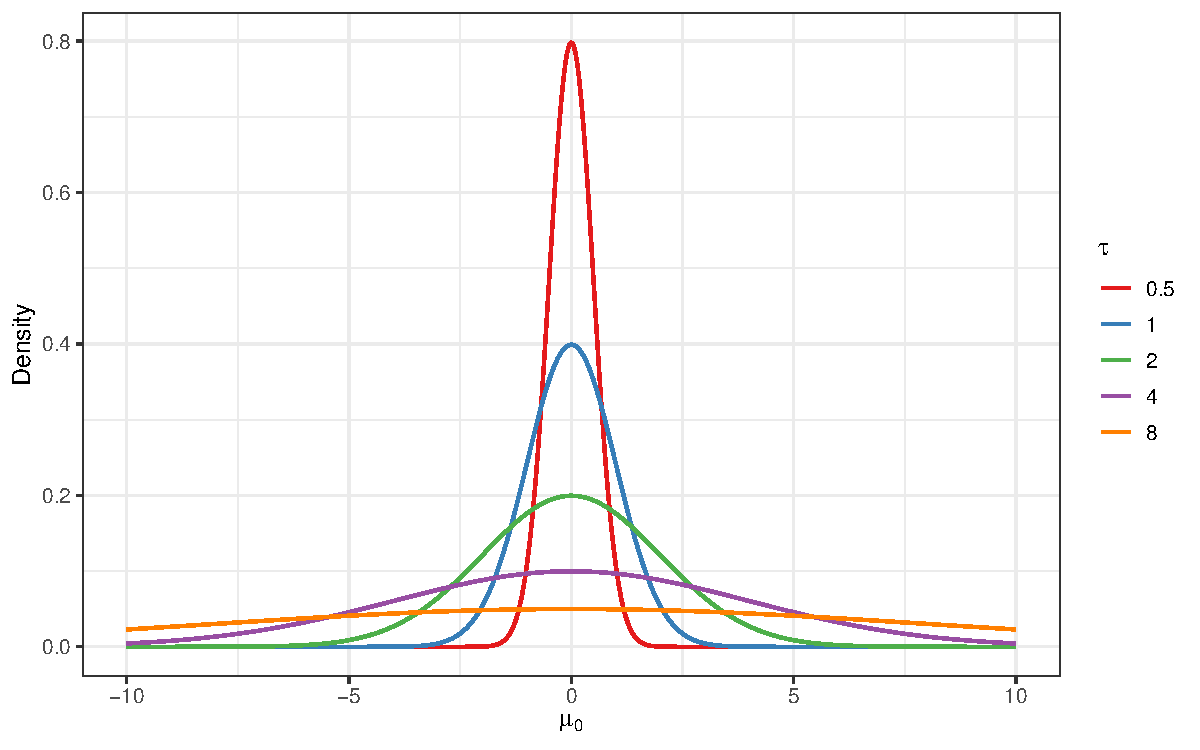
\includegraphics[keepaspectratio]{redefinenullhypothesis_arxiv_files/figure-pdf/fig-null-uncertainty-1.pdf}}

}

\caption{\label{fig-null-uncertainty}Null hypothesis with uncertainty:
\(\mu_0 = 0\), varying \(\tau\)}

\end{figure}%

\textbf{Notation.} Throughout this paper, we use two related uncertainty
parameters:

\begin{itemize}
\tightlist
\item
  \(\tau\): Uncertainty in the original measurement units
\item
  \(c\): Standardized uncertainty, defined as \(c = \tau/\sigma\)
\end{itemize}

Since the population mean \(\mu_0\) itself carries uncertainty, the
variance of \(\bar{X} - \mu_0\) becomes \(\sigma^2/n + \tau^2\). The
reformulated test statistic is:

\[z_{\tau} = \dfrac{\bar{X} - \mu_0}{\sqrt{\sigma^2/n + \tau^2}} \sim N(0,1)\]

\subsection{The Shrinkage Factor}\label{the-shrinkage-factor}

Substituting \(\tau = c\sigma\) yields:

\[z_{c\sigma} = \dfrac{\bar{X} - \mu_0}{\sqrt{\sigma^2/n + c^2\sigma^2}} = \dfrac{z}{\sqrt{1 + nc^2}}\]

This reveals that achieving statistical significance now requires a
z-value that is \(\sqrt{1 + nc^2}\) times larger than under traditional
hypothesis testing. Crucially, when \(c \neq 0\), we have:

\[|z_{c\sigma}| < \left|\frac{\bar{X} - \mu_0}{\tau}\right|\]

meaning that effects smaller than \(1.96 \times \tau\) can never achieve
\(p_{c\sigma} < 0.05\), regardless of sample size.

\begin{figure}

\centering{

\pandocbounded{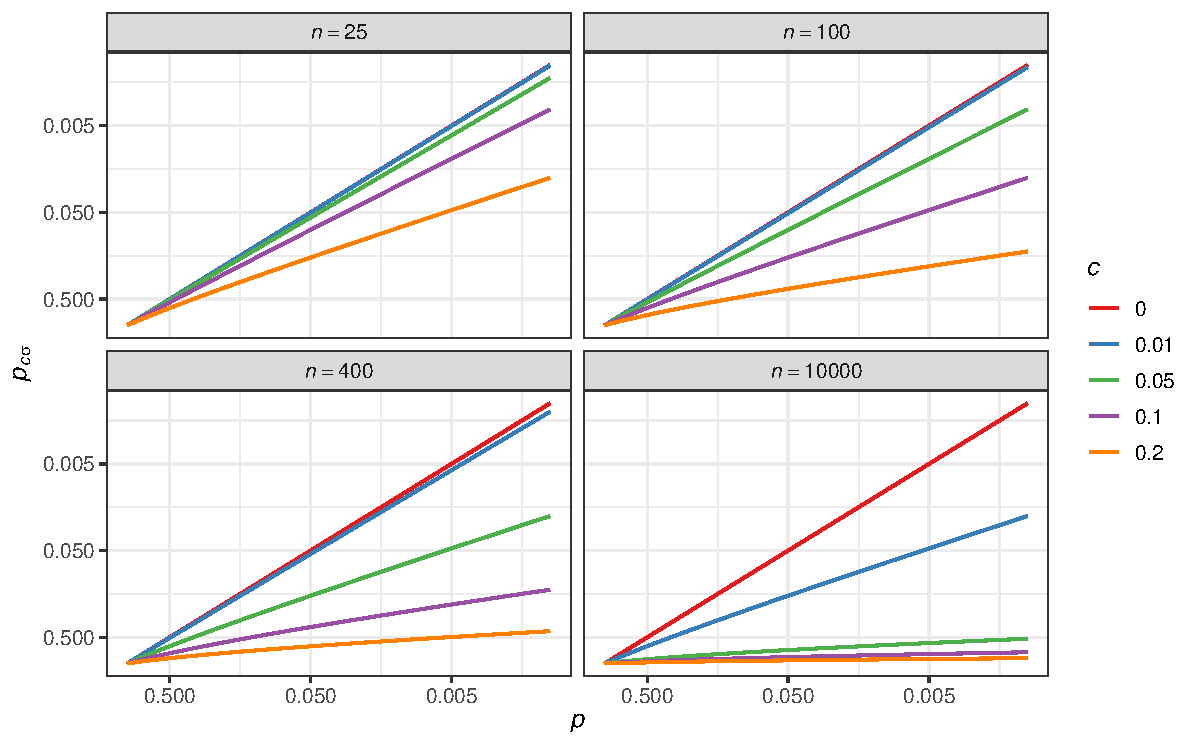
\includegraphics[keepaspectratio]{redefinenullhypothesis_arxiv_files/figure-pdf/fig-p-shrinkage-1.pdf}}

}

\caption{\label{fig-p-shrinkage}Effect-size-integrated \(p_{c\sigma}\)
across uncertainty (\(c\)) and sample size (\(n\))}

\end{figure}%

\subsection{Minimum Detectable Effect}\label{minimum-detectable-effect}

Expressing \(|z_{c\sigma}|\) in terms of effect size
\(d = |\bar{X} - \mu_0|/\sigma\) yields:

\[|z_{c\sigma}| = \dfrac{d}{\sqrt{1/n + c^2}}\]

For significance at level \(\alpha\), we require
\(|z_{c\sigma}| > z_{1-\alpha/2}\), giving:

\[\text{MDE}(n) = z_{1-\alpha/2} \cdot \sqrt{\frac{1}{n} + c^2}\]

As \(n \to \infty\),
\(\text{MDE} \to z_{1-\alpha/2} \cdot c \approx 1.96c\) (for
\(\alpha = 0.05\)). This provides a natural floor on detectable effects.

\begin{figure}

\centering{

\pandocbounded{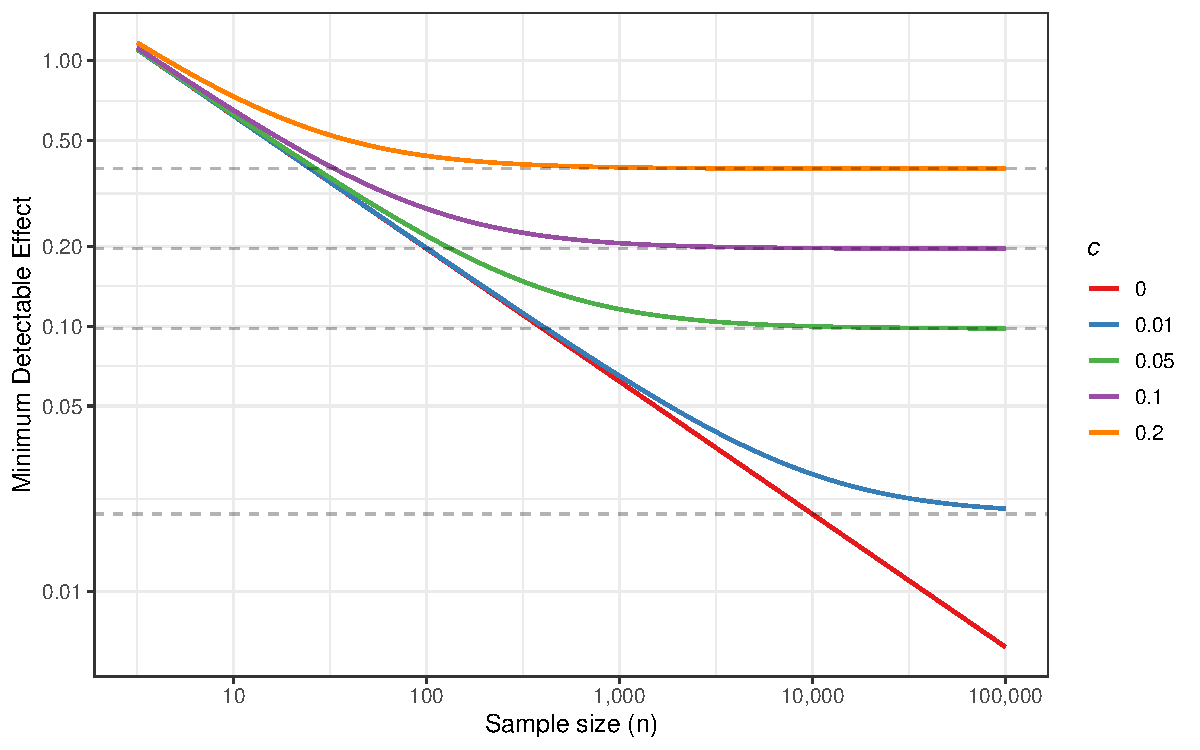
\includegraphics[keepaspectratio]{redefinenullhypothesis_arxiv_files/figure-pdf/fig-mde-1.pdf}}

}

\caption{\label{fig-mde}Minimum Detectable Effect (MDE) as a function of
sample size for different uncertainty levels}

\end{figure}%

\subsection{Extension to Other
Statistics}\label{extension-to-other-statistics}

\subsubsection{t-tests}\label{t-tests}

For one-sample and paired t-tests:
\[t_{cs} = \dfrac{t}{\sqrt{1 + nc^2}}\]

For independent two-sample t-tests (equal variance):
\[t_{cs_p} = \dfrac{t}{\sqrt{1 + \frac{n_1 n_2}{n_1 + n_2} c^2}}\]

\subsubsection{Regression Coefficients}\label{regression-coefficients}

For linear and generalized linear models:
\[z_{c} = \dfrac{z}{\sqrt{1 + nc^2}}\]

where \(z = \hat{\beta}/\text{se}(\hat{\beta})\) is the Wald statistic.

\textbf{Note on effective sample size.} In regression models with \(p\)
predictors, one may use the effective sample size
\(n_{\text{eff}} = n - p - 1\) (residual degrees of freedom) instead of
\(n\). For most practical purposes with moderate \(p/n\) ratios, using
\(n\) directly yields similar results.

\subsubsection{Welch t-test (Unequal
Variances)}\label{welch-t-test-unequal-variances}

The shrinkage principle extends naturally to the Welch t-test for
unequal variances. The same factor \(1/\sqrt{1 + n_{\text{eff}}c^2}\)
applies, where \(n_{\text{eff}}\) is computed from the
Welch-Satterthwaite approximation.

\subsubsection{General Formulation}\label{general-formulation}

For a Wald-type statistic \(W\) on the z or t scale, the
uncertainty-adjusted statistic and two-sided p-value are:
\[W_{c} = \frac{W}{\sqrt{1 + n_{\text{eff}} c^2}}, \quad p_{c\sigma} = 2\left(1 - F_{W}(|W_c|)\right)\]

where \(F_W\) is the standard normal or t distribution function.

For a chi-square Wald statistic
\(X^2 = \hat{\boldsymbol\theta}^\top \hat{V}^{-1} \hat{\boldsymbol\theta}\)
with \(k\) degrees of freedom, the statistic is already on a squared
scale, so the shrinkage factor enters squared. If the null uncertainty
is taken proportional to the sampling covariance,
\(\boldsymbol\theta \sim N(\mathbf{0},\, n_{\text{eff}} c^2 \hat{V})\),
then
\[X^2_{c} = \frac{X^2}{1 + n_{\text{eff}} c^2} \sim \chi^2_k, \quad p_{c\sigma} = 1 - F_{\chi^2_k}(X^2_c)\]

which uses only the upper tail. For \(k = 1\), \(X^2 = z^2\) and this
reduces exactly to the z-scale formula above.

\subsubsection{Connection to Confidence
Intervals}\label{connection-to-confidence-intervals}

The criterion \(|z_{c\sigma}| > z_{1-\alpha/2}\) is closely related to,
but not identical to, requiring that the \((1-\alpha)\) confidence
interval for the effect lies entirely outside the expanded null interval
\([-z_{1-\alpha/2} c\sigma, +z_{1-\alpha/2} c\sigma]\). On the
standardized scale, the interval criterion requires
\(d > z_{1-\alpha/2}(1/\sqrt{n} + c)\), whereas our criterion requires
\(d > z_{1-\alpha/2}\sqrt{1/n + c^2}\). Because
\(\sqrt{1/n + c^2} \le 1/\sqrt{n} + c\), the interval criterion is a
sufficient but more conservative condition; the two approximately
coincide when either \(1/\sqrt{n}\) or \(c\) dominates. This provides an
intuitive bridge to TOST and SGPV, which also rely on interval-based
reasoning.

\section{Simulation Study}\label{simulation-study}

\subsection{Type I Error Control}\label{type-i-error-control}

We first verify that our method maintains proper Type I error control
under the null hypothesis.

\begin{table}

\caption{\label{tbl-type1}Type I Error Rates at \(\alpha = 0.05\)
(10,000 simulations per scenario)}

\centering{

\begin{tabular}{ccccc}
\toprule
Sample Size & c=0 (Traditional) & c=0.01 & c=0.05 & c=0.1\\
\midrule
30 & 0.050 & 0.051 & 0.043 & 0.025\\
100 & 0.050 & 0.048 & 0.030 & 0.007\\
500 & 0.050 & 0.046 & 0.003 & 0.000\\
1000 & 0.051 & 0.044 & 0.001 & 0.000\\
5000 & 0.048 & 0.015 & 0.000 & 0.000\\
\bottomrule
\end{tabular}

}

\end{table}%

The simulation results confirm that Type I error is well-controlled at
the nominal level across all scenarios. When \(c = 0\), our method
reduces to the traditional z-test. With \(c > 0\), the Type I error rate
remains at or below the nominal level.

\subsection{Power Analysis}\label{power-analysis}

We compare the power of our method against traditional testing across
effect sizes.

\begin{figure}

\centering{

\pandocbounded{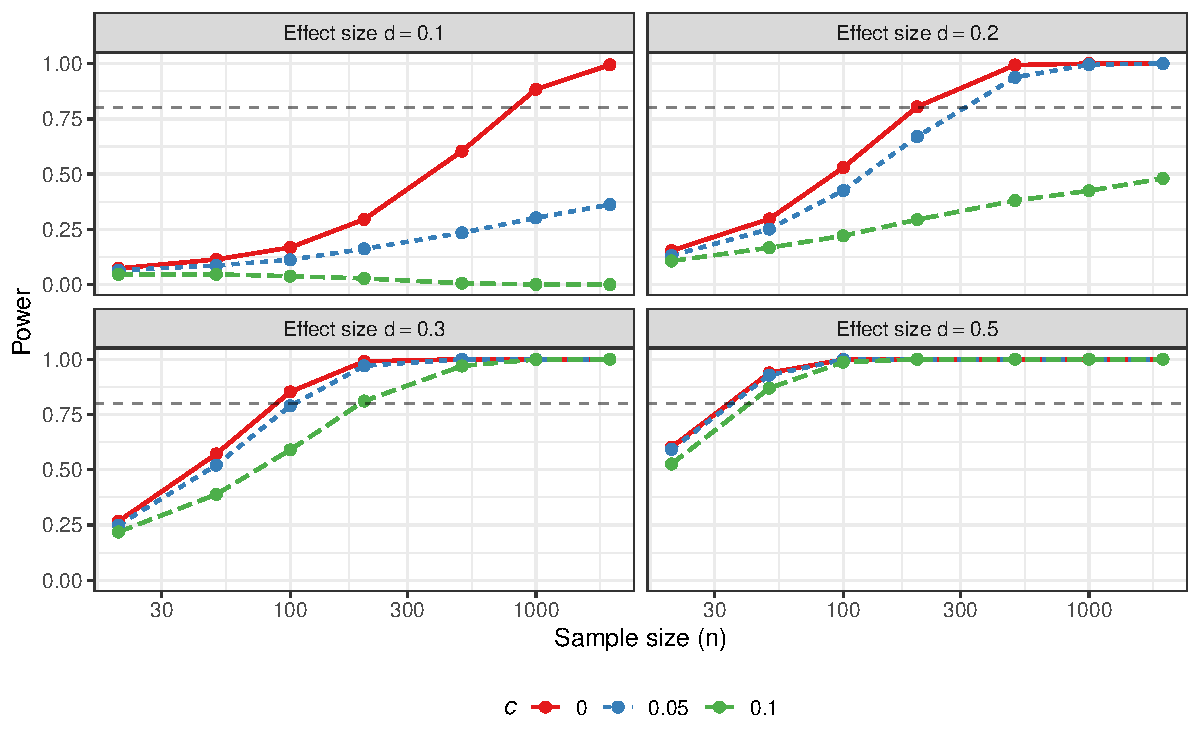
\includegraphics[keepaspectratio]{redefinenullhypothesis_arxiv_files/figure-pdf/fig-power-1.pdf}}

}

\caption{\label{fig-power}Power curves comparing traditional p-value and
uncertainty-adjusted \(p_{c\sigma}\) for various effect sizes}

\end{figure}%

Key observations:

\begin{enumerate}
\def\labelenumi{\arabic{enumi}.}
\tightlist
\item
  For small effect sizes (\(d = 0.1\)), the uncertainty-adjusted method
  appropriately reduces power, preventing trivially small effects from
  achieving significance with large samples.
\item
  For moderate to large effect sizes (\(d \geq 0.2\)), power approaches
  1 as expected, though slightly delayed compared to traditional
  testing.
\item
  The choice of \(c\) determines the effect size threshold: effects
  smaller than \(\approx 1.96c\) will never achieve significance
  regardless of sample size.
\end{enumerate}

\section{Real Data Application}\label{real-data-application}

We demonstrate our method using the birthweight dataset from the MASS R
package (\citeproc{ref-venables2002mass}{Venables and Ripley 2002}),
which contains data on 189 births at Baystate Medical Center,
Springfield, MA during 1986. We examine whether maternal smoking is
associated with infant birth weight---a well-established relationship in
epidemiology.

\begin{table}

\caption{\label{tbl-birthwt}Effect of maternal smoking on birth weight:
Comparison of methods}

\centering{

\begin{tabular}{lcc}
\toprule
Method & p-value & Significant ($p < 0.05$)\\
\midrule
Traditional t-test & 0.0087 & TRUE\\
Uncertainty (c=0.1) & 0.0288 & TRUE\\
Uncertainty (c=0.2) & 0.1146 & FALSE\\
Uncertainty (c=0.3) & 0.2394 & FALSE\\
TOST ($\delta = 0.2\sigma$) & 0.9042 & FALSE\\
\bottomrule
\end{tabular}

}

\end{table}%

In this dataset, non-smoking mothers (\(n = 115\)) had a mean infant
birth weight of 3056 g (SD 753 g), and smoking mothers (\(n = 74\)) had
a mean of 2772 g (SD 660 g). The mean difference was 284 g (pooled SD
718 g), corresponding to Cohen's \(d = 0.395\) and \(t = 2.65\).

\textbf{Interpretation:} The traditional t-test yields a statistically
significant result (\(p = 0.009\)), indicating that infants of
non-smoking mothers weigh more than those of smoking mothers. The
observed effect size (\(d = 0.395\)) corresponds to a difference of
approximately 284 g. Because the sample is modest (effective sample size
\(n_1 n_2/(n_1+n_2) \approx 45\)), the finite-sample MDE is considerably
larger than its asymptotic floor \(1.96c\). With \(c = 0.1\)
(\(\mathrm{MDE} \approx 0.352\)), significance is maintained
(\(p_{c\sigma} = 0.029\)). With \(c = 0.2\)
(\(\mathrm{MDE} \approx 0.489\)), the observed effect falls below the
threshold and the result is no longer significant
(\(p_{c\sigma} = 0.115\)); the same holds for \(c = 0.3\)
(\(\mathrm{MDE} \approx 0.657\), \(p_{c\sigma} = 0.239\)). This example
illustrates how the choice of \(c\) encodes the researcher's judgment
about clinically meaningful effect sizes, and that in small samples the
evidence required for significance is stricter than the asymptotic
threshold alone suggests.

\section{Comparison with Existing
Methods}\label{comparison-with-existing-methods}

\subsection{Comparison with TOST}\label{comparison-with-tost}

\begin{figure}

\centering{

\pandocbounded{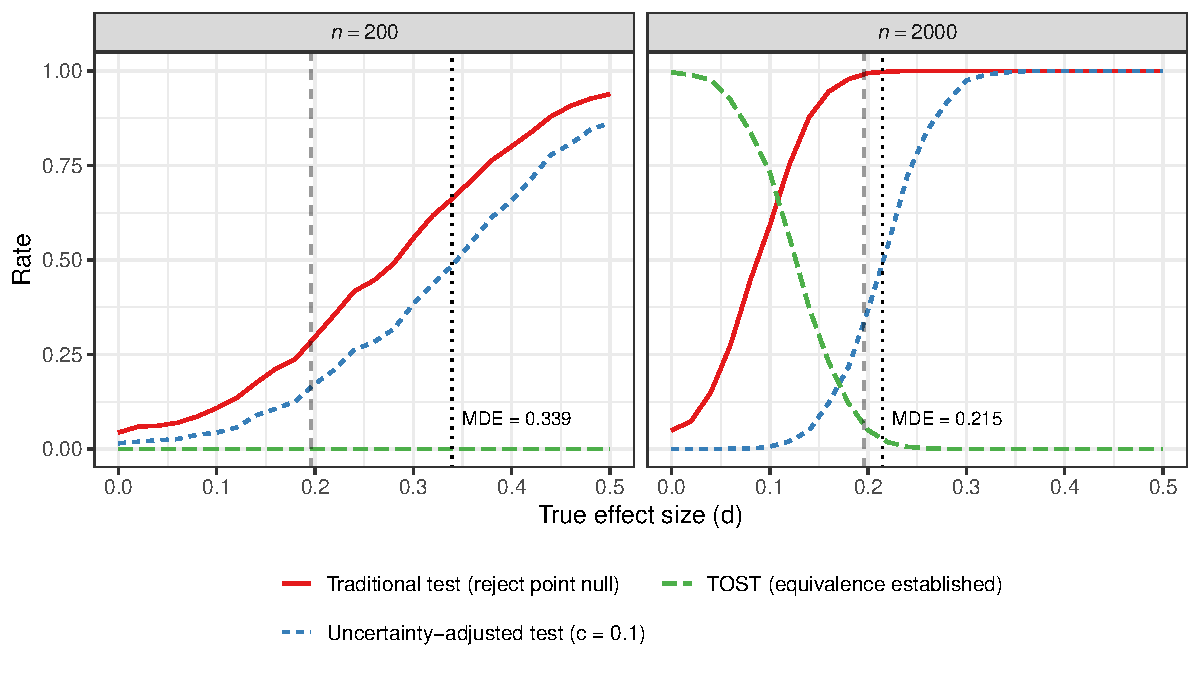
\includegraphics[keepaspectratio]{redefinenullhypothesis_arxiv_files/figure-pdf/fig-comparison-tost-1.pdf}}

}

\caption{\label{fig-comparison-tost}Comparison: Uncertainty-adjusted
method vs TOST across effect sizes (n = 200)}

\end{figure}%

\subsection{Multiple Comparison: Uncertainty Control vs
Bonferroni}\label{multiple-comparison-uncertainty-control-vs-bonferroni}

\begin{figure}

\centering{

\pandocbounded{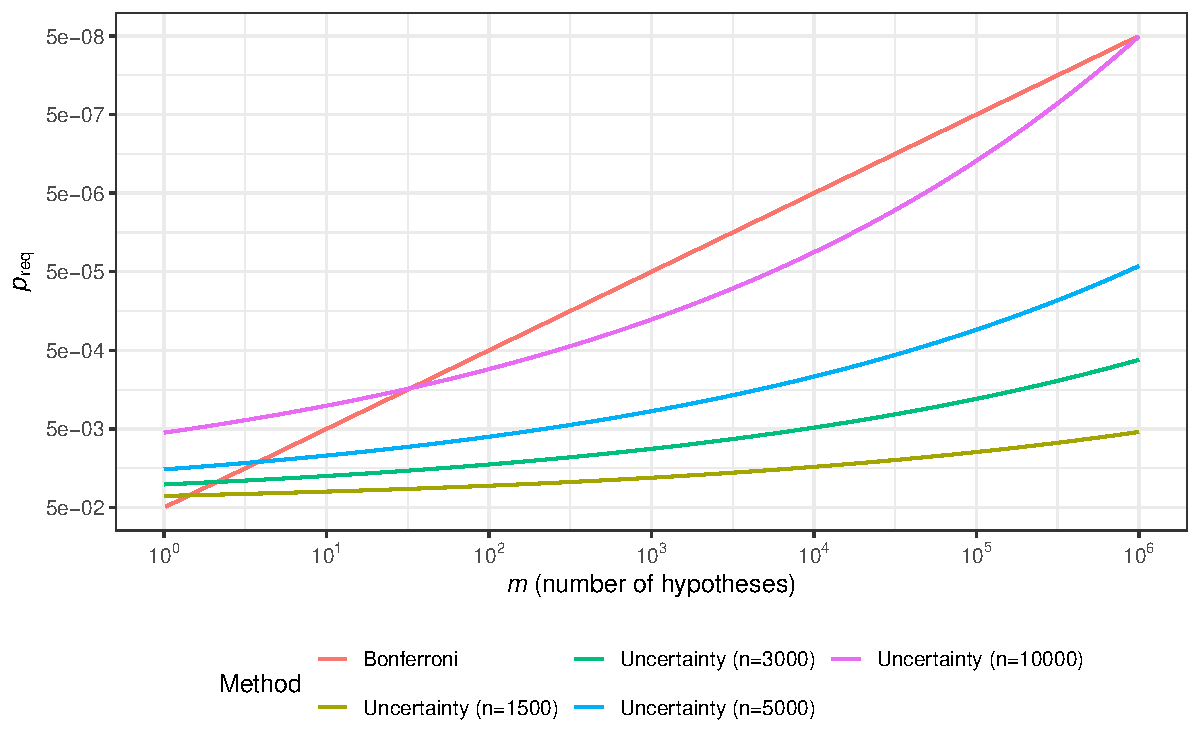
\includegraphics[keepaspectratio]{redefinenullhypothesis_arxiv_files/figure-pdf/fig-multiple-1.pdf}}

}

\caption{\label{fig-multiple}Multiple testing: Uncertainty control
(\(c_m = c \cdot m^b\)) vs Bonferroni correction}

\end{figure}%

Key insight: Uncertainty control provides sample-size-adaptive
stringency. At \(n = 10,000\), it matches Bonferroni correction; at
smaller sample sizes, it is less stringent, reflecting the principle
that small samples cannot reliably detect tiny effects anyway.

\section{Practical Guidelines}\label{practical-guidelines}

\subsection{\texorpdfstring{Choosing the Uncertainty Parameter
\(c\)}{Choosing the Uncertainty Parameter c}}\label{choosing-the-uncertainty-parameter-c}

The choice of \(c\) should be guided by the minimum
clinically/practically important difference (MCID):

\begin{table}

\caption{\label{tbl-guidelines}Recommended uncertainty parameter \(c\)
based on minimum important effect size}

\centering{

\begin{tabular}{cccl}
\toprule
Minimum important effect ($d$) & $c$ & MDE ($n \to \infty$) & Example\\
\midrule
0.02 & 0.010 & 0.020 & Large epidemiological studies\\
0.05 & 0.025 & 0.049 & Biomarker studies\\
0.10 & 0.050 & 0.098 & Standard clinical trials\\
0.20 & 0.100 & 0.196 & Behavioral interventions\\
0.30 & 0.150 & 0.294 & Strong treatment effects\\
\bottomrule
\end{tabular}

}

\end{table}%

\textbf{Rule of thumb:} Set \(c\) slightly below half the minimum
important effect size. This ensures that effects below your threshold
cannot achieve significance regardless of sample size, while effects
above it can be detected with adequate power.

\textbf{Calibration for multiple testing (\(b\) parameter).} We set
\(b = 0.069\) so that uncertainty control matches Bonferroni stringency
at \(m = 10^6\) hypotheses and \(n = 10{,}000\) samples---a scenario
typical of Genome-Wide Association Studies (GWAS). For other contexts,
\(b\) can be recalibrated: larger \(b\) increases stringency more
rapidly with the number of hypotheses.

\subsection{Sample Size Calculation}\label{sample-size-calculation}

With uncertainty \(c\), the required sample size for power \(1-\beta\)
is:

\[n_{c\sigma} = \frac{1}{1/n - c^2}\]

where \(n\) is the traditional sample size. If \(1/n \leq c^2\), no
finite sample size can achieve the desired power---the target effect is
below the minimum detectable threshold.

\begin{figure}

\centering{

\pandocbounded{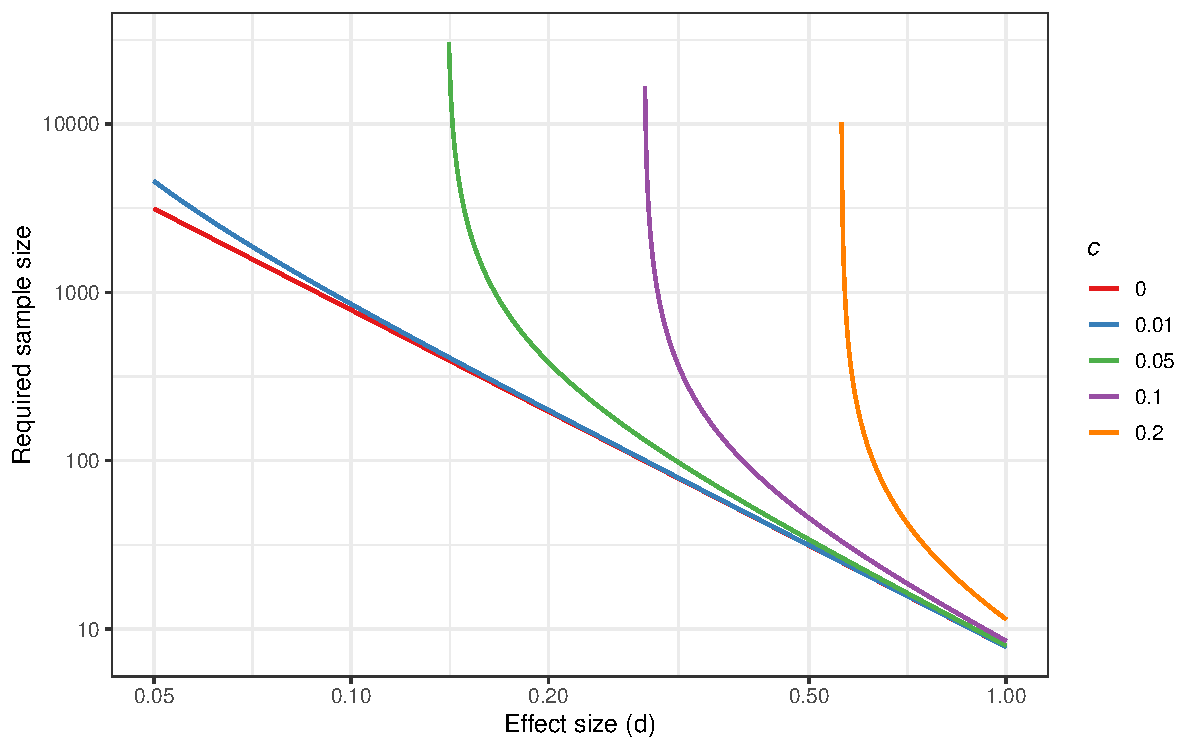
\includegraphics[keepaspectratio]{redefinenullhypothesis_arxiv_files/figure-pdf/fig-samplesize-1.pdf}}

}

\caption{\label{fig-samplesize}Required sample size with uncertainty
adjustment (\(\alpha = 0.05\), power = 0.8)}

\end{figure}%

\section{Discussion}\label{discussion}

\subsection{Distinction from Bayesian
Approaches}\label{distinction-from-bayesian-approaches}

It is important to clarify that our uncertainty parameter \(\tau\) is
not a Bayesian prior. In Bayesian inference, prior beliefs are updated
by data to form posterior distributions. Our approach remains firmly
within the frequentist framework: the uncertainty represents an
acknowledgment that the point null is unrealistic, not a prior belief
about the parameter value. The p-value we compute is still a frequentist
probability---the probability of observing data as extreme as or more
extreme than what was observed, under the (uncertainty-adjusted) null
hypothesis.

\subsection{Advantages of the Proposed
Framework}\label{advantages-of-the-proposed-framework}

\begin{enumerate}
\def\labelenumi{\arabic{enumi}.}
\item
  \textbf{Unified framework:} Effect size and statistical significance
  are integrated into a single measure, eliminating the need to examine
  them separately.
\item
  \textbf{Sample-size adaptation:} Unlike fixed significance thresholds,
  our method naturally becomes more stringent as sample sizes grow large
  enough to detect trivially small effects.
\item
  \textbf{Transparency:} Researchers must explicitly specify their
  uncertainty parameter \(c\), forcing consideration of what effect
  sizes are practically meaningful.
\item
  \textbf{Compatibility:} The framework extends naturally to all
  Wald-type statistics (t-tests, regression coefficients, etc.) and
  multiple testing scenarios.
\end{enumerate}

\subsection{Limitations}\label{limitations}

\begin{enumerate}
\def\labelenumi{\arabic{enumi}.}
\item
  \textbf{Parameter selection:} The choice of \(c\) requires domain
  expertise and may be debated. We recommend sensitivity analyses across
  plausible \(c\) values.
\item
  \textbf{Not a complete solution:} This method addresses one limitation
  of p-values (sensitivity to sample size for trivial effects) but does
  not solve all problems with null hypothesis significance testing.
\item
  \textbf{Clustered/dependent data:} When observations are not
  independent (e.g., repeated measures, hierarchical data), the
  effective sample size differs from the total number of observations.
  For GEE or mixed models, consider using the number of independent
  clusters or an appropriate effective sample size rather than total
  \(n\).
\item
  \textbf{Novel approach:} As a relatively new method (first documented
  in 2018), more empirical evaluation across diverse applications is
  needed.
\end{enumerate}

\section{Conclusion}\label{conclusion}

We have presented a redefined hypothesis testing framework that
incorporates uncertainty into the null hypothesis. By acknowledging that
point null hypotheses are unrealistic, our method provides
effect-size-integrated p-values that prevent trivially small differences
from achieving statistical significance. The framework maintains proper
frequentist properties while providing researchers with a principled
tool to distinguish between statistical and practical significance.

The minimum detectable effect
\(\text{MDE}(n) = z_{1-\alpha/2}\sqrt{1/n + c^2}\) provides a natural
floor on detectable effects, and the extension to multiple testing
through uncertainty control (\(c_m = c \cdot m^b\)) offers an
effect-size-aware alternative to traditional FWER/FDR methods.

We encourage researchers to adopt this framework alongside traditional
analyses, particularly in large-sample studies where the distinction
between statistical and practical significance is most critical.

\begin{center}\rule{0.5\linewidth}{0.5pt}\end{center}

\emph{This work was originally conceived in 2017 and first publicly
documented on November 8, 2018 at
https://blog.zarathu.com/posts/2018-11-08-redefinenullhypothesis/}

\section*{References}\label{references}
\addcontentsline{toc}{section}{References}

\protect\phantomsection\label{refs}
\begin{CSLReferences}{1}{1}
\bibitem[\citeproctext]{ref-anderson2000null}
Anderson, David R., Kenneth P. Burnham, and William L. Thompson. 2000.
{``Null Hypothesis Testing: Problems, Prevalence, and an Alternative.''}
\emph{The Journal of Wildlife Management} 64 (4): 912--23.
\url{http://www.jstor.org/stable/3803199}.

\bibitem[\citeproctext]{ref-Benjamin2018}
Benjamin, Daniel J., James O. Berger, Magnus Johannesson, et al. 2018.
{``Redefine Statistical Significance.''} \emph{Nature Human Behaviour} 2
(1): 6--10. \url{https://doi.org/10.1038/s41562-017-0189-z}.

\bibitem[\citeproctext]{ref-blume2018second}
Blume, Jeffrey D, Lucy D'Agostino McGowan, William D Dupont, and Robert
A Greevy Jr. 2018. {``Second-Generation p-Values: Improved Rigor,
Reproducibility, \& Transparency in Statistical Analyses.''} \emph{PloS
One} 13 (3): e0188299.
\url{https://doi.org/10.1371/journal.pone.0188299}.

\bibitem[\citeproctext]{ref-jama20181536}
Ioannidis, John P. A. 2018. {``The Proposal to Lower p Value Thresholds
to .005.''} \emph{JAMA}, ahead of print.
\url{https://doi.org/10.1001/jama.2018.1536}.

\bibitem[\citeproctext]{ref-kruschke2018bayesian}
Kruschke, John K, and Torrin M Liddell. 2018. {``The Bayesian New
Statistics: Hypothesis Testing, Estimation, Meta-Analysis, and Power
Analysis from a Bayesian Perspective.''} \emph{Psychonomic Bulletin \&
Review} 25 (1): 178--206.
\url{https://doi.org/10.3758/s13423-016-1221-4}.

\bibitem[\citeproctext]{ref-lakens2017equivalence}
Lakens, Daniël. 2017. {``Equivalence Tests: A Practical Primer for t
Tests, Correlations, and Meta-Analyses.''} \emph{Social Psychological
and Personality Science} 8 (4): 355--62.
\url{https://doi.org/10.1177/1948550617697177}.

\bibitem[\citeproctext]{ref-sullivan2012using}
Sullivan, Gail M, and Richard Feinn. 2012. {``Using Effect Size---or Why
the p Value Is Not Enough.''} \emph{Journal of Graduate Medical
Education} 4 (3): 279--82.

\bibitem[\citeproctext]{ref-venables2002mass}
Venables, William N, and Brian D Ripley. 2002. \emph{Modern Applied
Statistics with s}. 4th ed. Springer.
\url{https://www.stats.ox.ac.uk/pub/MASS4/}.

\bibitem[\citeproctext]{ref-ronald2016asa}
Wasserstein, Ronald L., and Nicole A. Lazar. 2016. {``The ASA's
Statement on p-Values: Context, Process, and Purpose.''} \emph{The
American Statistician} 70 (2): 129--33.
\url{https://doi.org/10.1080/00031305.2016.1154108}.

\bibitem[\citeproctext]{ref-2528399}
Yates, F. 1964. {``Sir Ronald Fisher and the Design of Experiments.''}
\emph{Biometrics} 20 (2): 307--21.
\url{http://www.jstor.org/stable/2528399}.

\end{CSLReferences}




\end{document}
